\section{Введение}

\textbf{Цель работы:}
1) измерение температурной зависимости  коэффициента поверхностного натяжения дистиллированной воды с использованием известного коэффициента поверхностного натяжения спирта;  2) определение полной поверхностной энергии  и теплоты, необходимой для изотермического образования единицы  поверхности жидкости  при различной температуре.

\textbf{В работе используются:}
прибор  Ребиндера  с термостатом и микроманометром; исследуемые жидкости; стаканы.

Наличие поверхностного слоя приводит к различию давлений по разные стороны от искривленной границы раздела двух сред.  Для сферического пузырька с воздухом  внутри жидкости избыточное давление даётся формулой Лапласа:
\begin{equation}
    \Delta P = P_\text{внутри} - P_\text{снаружи} = \frac{2\sigma}{r},
    \label{equ:laplas}
\end{equation}
где $\sigma$ –- коэффициент поверхностного натяжения, $P_\text{внутри}$ и $P_\text{снаружи}$ –- давление внутри пузырька и снаружи, $r$ –- радиус кривизны поверхности раздела двух фаз. Эта формула лежит в основе предлагаемого метода определения коэффициента поверхностного натяжения жидкости. Измеряется давление $\Delta P$, необходимое для выталкивания в жидкость пузырька воздуха.

\textbf{Экспериментальная установка.} Исследуемая жидкость (дистиллированная вода) наливается в сосуд (колбу) В (рис. \ref*{pic:p1}). Тестовая жидкость  (этиловый спирт) наливается  в сосуд Е.  При измерениях  колбы герметично закрываются  пробками.   Через одну из двух пробок  проходит полая металлическая игла С. Этой пробкой закрывается сосуд, в котором  проводятся измерения. Верхний конец иглы открыт в атмосферу, а нижний погружен в жидкость. Другой сосуд герметично закрывается второй пробкой. При создании достаточного  разряжения воздуха в колбе с иглой пузырьки воздуха начинают пробулькивать через жидкость. Поверхностное натяжение можно определить по величине разряжения $\Delta P$ (\ref*{equ:laplas}), необходимого для прохождения пузырьков (при известном радиусе иглы).

\begin{figure}[h]
    \centering
    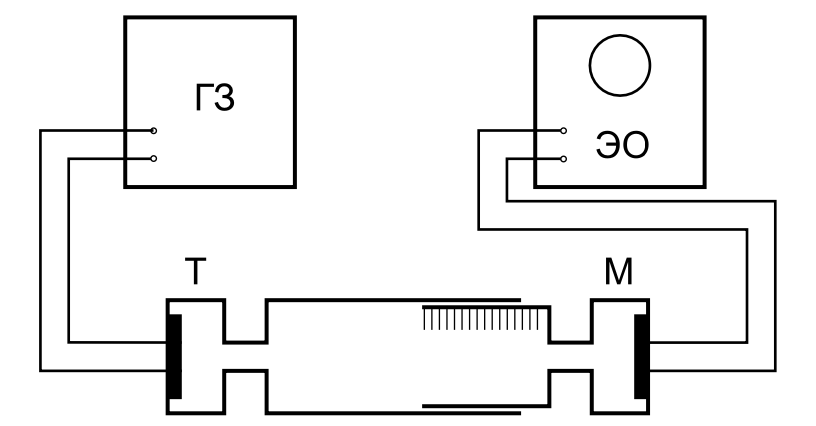
\includegraphics[width = 0.5\linewidth]{p1.png}
    \caption{Схема установки для измерения температурной зависимости коэффициента поверхностного натяжения.}
    \label{pic:p1}
\end{figure}

Разряжение в системе создается с помощью аспиратора А. Кран К$_2$ разделяет две полости аспиратора. Верхняя полость при закрытом кране К$_2$ заполняется водой. Затем кран К$_2$ открывают и заполняют водой  нижнюю полость  аспиратора.  Разряжение воздуха создается в нижней полости  при открывании крана К$_1$, когда  вода вытекает из неё по каплям. В колбах В и С, соединённых трубками с нижней полостью аспиратора,  создается такое же пониженное давление. Разность давлений в полостях с разряженным воздухом и атмосферой измеряется спиртовым микроманометром.

Для стабилизации температуры исследуемой жидкости через рубашку D колбы В непрерывно прогоняется вода из термостата.

Обычно кончик иглы лишь касается поверхности жидкости, чтобы исключить влияние гидростатического давления столба жидкости. Однако при измерении температурной зависимости коэффициента поверхностного натяжения возникает ряд сложностей. Во-первых, большая теплопроводность металлической трубки приводит к тому, что температура на конце трубки заметно ниже, чем в глубине жидкости. Во-вторых, тепловое расширение поднимает уровень жидкости при увеличении температуры.

Обе погрешности можно устранить, погрузив кончик трубки до самого дна. Полное давление, измеренное при этом микроманометром, $P = \Delta P + \rho g h$. Заметим, что $\rho gh$ от температуры практически не зависит, так как подъём уровня жидкости компенсируется уменьшением её плотности (произведение $\rho h$ определяется массой всей жидкости и поэтому постоянно). Величину $\rho gh$ следует измерить двумя способами. Во-первых, замерить величину $P_1 = \Delta P'$, когда кончик трубки только касается поверхности жидкости. Затем при этой же температуре опустить иглу до дна и замерить $P_2 = \rho gh + \Delta P''$. Из-за  несжимаемости  жидкости можно положить $\Delta P' = \Delta P''$ и тогда $\rho gh = P_2 - P_1$. Во-вторых, при измерениях $P_1$ и $P_2$ замерить линейкой  глубину погружения иглы $h$. Это можно сделать, замеряя расстояние между верхним концом иглы и любой неподвижной частью прибора при положении иглы на поверхности и в глубине колбы.

